\documentclass[language=german,style=solution]{smo}

\usepackage{tikz}

\title{SMO - Vorrunde 2016 - Lösungen}

\begin{document}

\begin{enumerate}

\item[\textbf{1.}] 
Zwei Kreise $k_1$ und $k_2$ schneiden sich in den Punkten $A$ und $C$. Sei $B$ der zweite Schnittpunkt von $k_1$ und der Tangente an $k_2$ in $A$, und sei $D$ der zweite Schnittpunkt von $k_2$ und der Tangente an $k_1$ in $C$. Zeige, dass $AD$ und $BC$ parallel sind.

\textbf{Lösung}

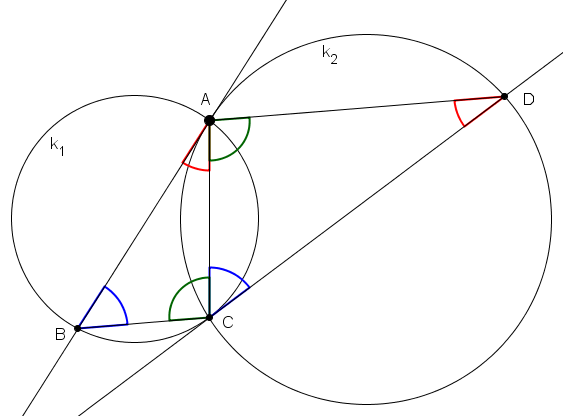
\includegraphics{muloe_2016_aufgabe1.png}

Nach dem Tangentenwinkelsatz gilt sowohl $\angle BAC=\angle ADC$ als auch $\angle CBA=\angle DCA$. Die beiden Dreiecke $ABC$ und $ACD$ stimmen also in zwei Winkeln überein und somit auch im dritten. Wir erhalten $\angle ACB=\angle CAD$, woraus sofort folgt, dass diese Winkel Wechselwinkel und $AD$ und $BC$ parallel sind.

\textbf{Marking Scheme}
\begin{itemize}
\item +1 für $\angle BAC=\angle ADC$
\item +1 für $\angle CBA=\angle DCA$
\item +1 für $\angle ACB=\angle CAD$
\end{itemize}

\newpage

\item[\textbf{2.}] 
Cunégonde a $n$ blocs de hauteur 1 à $n$ et souhaiterait les agencer, les uns après les autres, de telle manière que son chat puisse se déplacer en sautant d'un bloc à l'autre, de la gauche vers la droite. Son chat peut sauter d'un bloc au suivant si celui-ci est soit moins haut, soit plus haut de 1 que le bloc précédent. Au début, son chat se trouve sur le bloc à l'extrémité gauche.\\
De combien de manières Cunégonde peut-elle agencer ses blocs, pour que son chat puisse franchir tous les blocs ?

\textbf{Solution 1:}

Supposons que Cunégonde place le bloc de hauteur $n$ à la position $k$. Alors le bloc à la position $k-1$ dois avoir la hauteur $n-1$. En continuant comme ça, on voit que les $k$ premiers blocs doivent être $n-k+1, n-k+2, \dots , n$. Il nous reste ensuite les $n-k$ premiers blocs à placer sur $n-k$ positions. On répétant l'argument on voit que toutes les solutions s'obtiennent en plaçant les blocs par ordre décroissant puis en séparant les $n$ blocs en sous-ensembles de blocs consécutifs, dans lesquels on inverse l'ordre. \\
On peut obtenir chaque partition des $n$ blocs en sous-ensemble de blocs consécutifs par placer des traits enter les nombres. Par exemple $1 \ 2\ |\ 3 \ |\ 4\ 5$ correspond à la partition $[1,2][3][4,5]$. Comme on a $n-1$ espaces entre les nombres $1,2,\dots,n$ et pour chaque espace on peut placer un trait ou pas, on voit qu'il y a $2^{n-1}$ différentes partitions. Donc Cunégonde a $2^{n-1}$ possibilités d'agencer les $n$ blocs.

\textbf{Lösung 2:}

Man bemerkt, dass wenn die Katze beim Block der Höhe $k$ startet, sie zum höchsten Block hochlaufen muss, bevor sie runterspringen kann. Wenn sie das nicht macht, schafft sie es nicht mehr zum höchsten Block hoch, da $k$ gebraucht wurde und es zwischen $k - 1$ und $k + 1$ eine Lücke der Höhe $2$ gibt. Nun hat man die Blöcke von $1$ bis $k - 1$ übrig, für diese gilt wieder dasselbe Argument.\\  
Man stellt die Blöcke der Höhe $1$ bis $n$ der Reihe nach auf. Wenn die Blöcke $1$ bis $n - 1$ bereits aufgestellt sind, gibt es genau zwei Möglichkeiten, wo man $n$ noch hinstellen kann, und zwar hinter den Block mit Höhe $n - 1$ oder ganz an den Anfang.\\
Für den ersten Block gibt es eine Möglichkeit, für jeden weiteren zwei. Somit gibt es für $n$ Blöcke $2^{n-1}$ Möglichkeiten.

\textbf{Marking Scheme:}

\begin{itemize}
\item + 1 Wenn man sieht, dass die Klötze als eine absteigende Folge von aufsteigenden Partionen angeordnet sein muss.
\item Volle Punktzahl für korrekte Lösung
\item - 1 Wenn Induktion verwendet wird (wenn man von $n$ auf $n+1$ schliesst), aber die Verankerung unvollstäding ist (also der Fall $n = 1$ nicht angeschaut wurde). Oder wenn der Schritt von $n$ zu $n+1$ nicht klar erklärt wurde.
\item - 1 Wenn die Lösung nicht explizit hingeschrieben wurde.
\end{itemize}

\newpage

\item[\textbf{3.}]

Déterminer tous les entiers naturels $n$ tels que pour chaque diviseur positif $d$ de $n$ on ait 
\[
d+1 \div n+1.
\]

\textbf{Lösung:}
Pour tout nombre naturel $n$, $1$ est un diviseur de $n$ donc nous avons $2 \div n+1$. Ainsi $n$ doit être impair.

Si $n=1$, $d = 1$ est le seul diviseur de $n$ et clairement $2 \div 2$ donc $1$ est solution.

Sinon soit $p$ le plus petit facteur premier de $n$. Comme $p$ divise $n$ nous avons aussi $\frac{n}{p}$ divise $n$ et donc 
\[
\frac{n}{p}+1 \div n+1\quad \Rightarrow\quad \frac{n}{p}+1 \,\Big|\, p\left(\frac{n}{p}+1\right) - (n+1) = p-1
\]
Or, comme $p$ est le plus petit facteur premier de $n$, si $n\neq p$ nous avons alors d'une part $p\leq \frac{n}{p}$, d'autre part, par la relation de divisibilité trouvée ci-dessus, $\frac{n}{p}+1\leq p-1$, ce qui est une contradiction.

Les seules solutions possibles sont donc $n=1$ ou $n = p$ avec $p$ un nombre premier impair. On voit facilement que ce sont tous des solutions car les seuls diviseurs de $p$ sont $1$ et $p$ et comme $p$ est impair nous avons bien $2 \div p+1$ et $p+1 \div p+1$.

\textbf{Marking Scheme:}

\begin{itemize}
\item Prouver que $n$ est impair: 2 pts
\item Prouver que $n$ a au plus un facteur premier: 4 pts
\item Vérifier les solutions: 1 pts
\end{itemize}
Points partiels:
\begin{itemize}
\item Prouver une relation de divisibilité utile: 2 pts
\item Oublier que 1 est solution: -1 pt
\item Oublier que 2 est premier et pair: -1 pt
\end{itemize}

\newpage

\item[\textbf{4.}] 

Bei 22 Mathematikwettbewerben werden jeweils 5 Preise verteilt. Nachdem alle Wettbewerbe durchgeführt sind, bemerken die Organisatoren, dass es für jede Kombination von zwei Wett\-bewer\-ben genau einen gemeinsamen Preisträger gibt. Zeige, dass ein Teilnehmer bei allen Wettbe\-wer\-ben einen Preis gewonnen hat.

\textbf{Lösung 1:}

Wir betrachten einen Wettbewerb. In jedem anderen Wettbewerb muss einer der fünf Preisträger auch auf der Preisträgerliste stehen. Da es noch 21 andere Wettbewerbe gibt, muss mindestens einer der fünf Gewinner noch in mindestens fünf anderen Wettbewerben auch unter den besten fünf Schülern sein. Dass heisst es gibt einen Schüler Max, welcher an mindestens sechs Wettbewerben einen Preis gewann. 
Wir betrachten nun einen Wettbewerb A bei dem Max keinen Preis gewann, wir können annehmen, dass es denn gibt, da wir sonst fertig sind. Zusätzlich betrachen wir sechs der Wettbewerbe, bei denen Max gewann. Aus der Vorraussetzung folgt, dass je zwei dieser sechs Wettbewerbe keinen gemeinsamen Preisträger ausser Max haben. Der Wettbewerb A muss mit jedem dieser sechs Wettbewerbe einen gemeinsamen Preisträger haben. Da dies aber nicht Max sein kann, kann der Wettbewerb A aber maximal mit fünf der sechs Wettbewerbe einen gemeinsamen Preisträger haben, da die anderen vier Preisträger bei jedem der sechs Wettbewerbe komplett verschieden sind. Das ist ein Widerspruch zur Vorraussetzung und somit gibt es keinen Wettbewerb bei dem Max nicht auf der Preisträgerliste steht.

\textbf{Marking Scheme:}
\begin{itemize}
\item +2 Ein Teilnehmer, welcher bei min. 6 Wettbewerben auf der Preisliste steht.
\item +1 Die anderen Teilnehmer dieser 6 oder mehr Wettbewerben sind komplett disjunkt.
\item +3 Wenn ein Teilnehmer bei min. 6 Wettbewerben gewann, dann bei jedem anderen auch.
\item +1 Vollständigkeit
\item -1 kleine Fehler
\end{itemize}

\newpage
\textbf{Lösung 2:}

Wir nehmen an, dass nicht alle einen einzelnen gemeinsamen Preisträger haben. Daher muss es drei Menge $A,B,C$ geben, welche keinen gemeinsamen Preisträger haben. Das heisst:
\begin{gather*}
A\cap B={s_1}\\
A\cap C={s_2}\\
B\cap C={s_3}
\end{gather*}

Die Mengen sehen also so aus:
\begin{gather*}
A={s_1,s_2,a_1,a_2,a_3}\\
B={s_1,s_3,b_1,b_2,b_3}\\
C={s_2,s_3,c_1,c_2,c_3}
\end{gather*}

Wir zählen nun, an wievielen Wettbewerben die Preisträger aus $A$ noch gewonnen haben können. Da jeder Wettbewerb mit $A$ einen gemeinsam hat, haben wir so alle Wettbewerbe gezählt. Wir können zeigen, dass wir maximal 21 Wettbewerbe bekommen können.

Wenn wir den Teilnehmer $s_1$ betrachten, dann kann er höchstens an 3 anderen Wettbewerben gewonnen haben. Denn jeder Wettbewerb muss einen anderen Teilnehmer aus der Menge $C$ enthalten. Dafür kommen aber nur $c_1,c_2,c_3$ in Frage, denn $s_2,s_3$ haben bereits einen gemeinsamen Wettbewerb mit $s_1$.

Analog für $s_2$ mit den anderen Teilnehmern in der Menge $B$.

Wenn wir den Teilnehmer $a_1$ betrachten, dann kann er höchstens an 4 andere Wettbewerben gewonnen haben. Argument wie oben, aber es kommen $b_1,b_2,b_3,s_3$ aus der Menge $B$ in Frage.

Analog für $a_2,a_3$.

Wir zählen nun die Mengen, welche wir ohne einen einzelnen Preisträger konstruieren können:
\begin{enumerate}
\item 3 vom Anfang (die Menge $A,B,C$)
\item $2\cdot 3$ mit $s_1,s_2$
\item $3\cdot 4$ mit $a_1,a_2,a_3$
\end{enumerate}

Und kommen so auf maximal 21 Mengen. Zu wenig, also muss unsere Annahme falsch gewesen sein. 

\textbf{Marking Scheme:}
\begin{itemize}
\item +1 Annahme, dass es drei Wettbewerbe ohne gemeinsamen Preisträger gibt, mit Beschreibung der Mengen.
\item +3 Zählen, wieviele mit $s_1, s_2, s_3$ möglich sind.
\item +3 Zählen, wieviele mit $a_1, a_2, a_3$ möglich sind.
\item -1 falls nicht fertig gemacht wurde oder kleine Fehler.
\end{itemize}

\newpage

\item[\textbf{5.}] 

Soit $ABC$ un triangle avec $AB < AC$. La bissectrice de $\angle BAC$ coupe le côté $BC$ en $D$. Soit $k$ le cercle qui passe par $D$ et qui est tangent aux segments $AC$ et $AB$ en $E$, respectivement $F$. Soit $G$ le deuxième point d'intersection de $k$ avec $BC$. Soit $S$ le point d'intersection de $EG$ et $DF$. Montrer que $AD$ est perpendiculaire à $BS$.

\textbf{Lösung:}

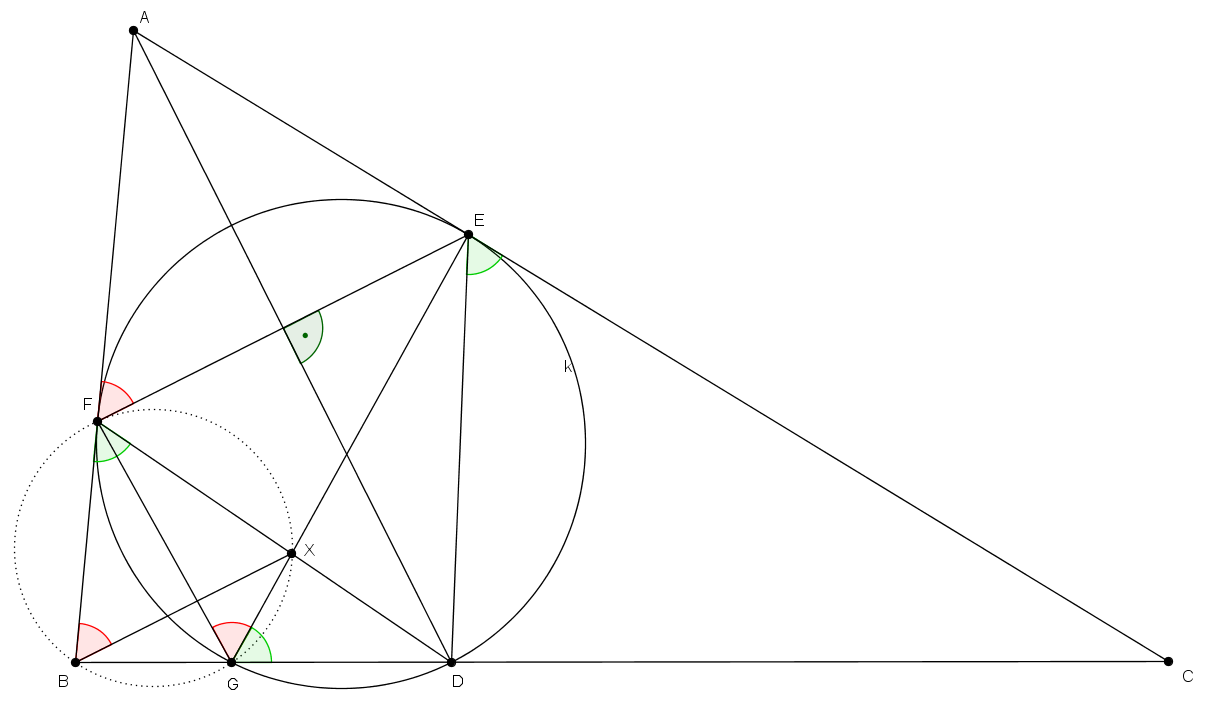
\includegraphics[width=\textwidth+1cm]{muloe_2016_aufgabe5.png}

Comme les points $E$ et $F$ sont symétriques par rapport à la droite $AD$,
\[
\angle AED = \angle DFA.
\]
Par la théorème de l'angle tangent,
\[
\angle EGD = \angle DEC.
\]
Or 
\[
\angle DEC = 180^{\circ}-\angle AED = 180^{\circ} - \angle DFA = \angle BFD,
\]
donc $\angle EGD = \angle BFD$ et
\[
\angle BGX + \angle BFX = (180^{\circ} - \angle EGD) + \angle BFD = 180^{\circ}.
\]

Ainsi le quadrilatère $BGXF$ est inscrit, donc
\[
\angle XBF = \angle XGF.
\]
Or, par la théorème de l'angle tangent,
\[
\angle EGF = \angle AFE.
\]
Ainsi
\[
\angle XBF = \angle EGF = \angle AFE,
\]
donc les droites $BX$ et $EF$ sont parallèles et, comme $EF\perp AD$ (symétrie), on en déduit que $BX\perp AD$.

\textbf{Marking Scheme:}

\begin{itemize}
\item +1 : $\triangle DEF$ isocèle
\item +3 : $BGSF$ inscrit
\item +1 : $\angle SBF = \angle EFA$
\item +2 : finir
\end{itemize}

\end{enumerate}

\end{document}
